
\newcommand{\CanTableNote}{$LEAP$ is the Longitudinal Employment Analysis Program and $CanSynLBD$ is the Canadian synthetic database based on LEAP. }

\subsection{Entity Characteristics}

\begin{figure}[t]
\begin{subfigure}[h]{0.48\linewidth}
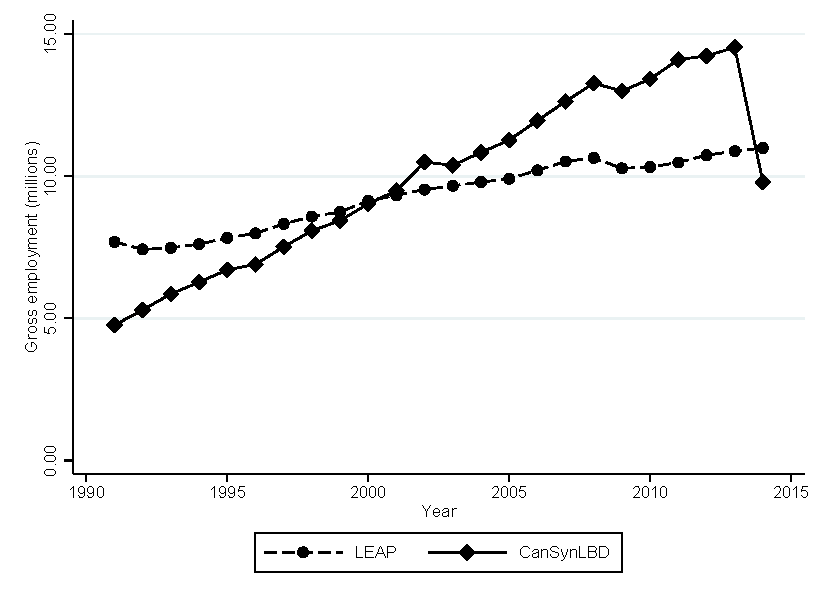
\includegraphics[trim=0 40 0 0,clip, width=\linewidth]{graphs/Gross_employment_level_by_year_private_bw.pdf}
%\caption{CanSynLBD}
\end{subfigure}
\hfill
\begin{subfigure}[h]{0.48\linewidth}
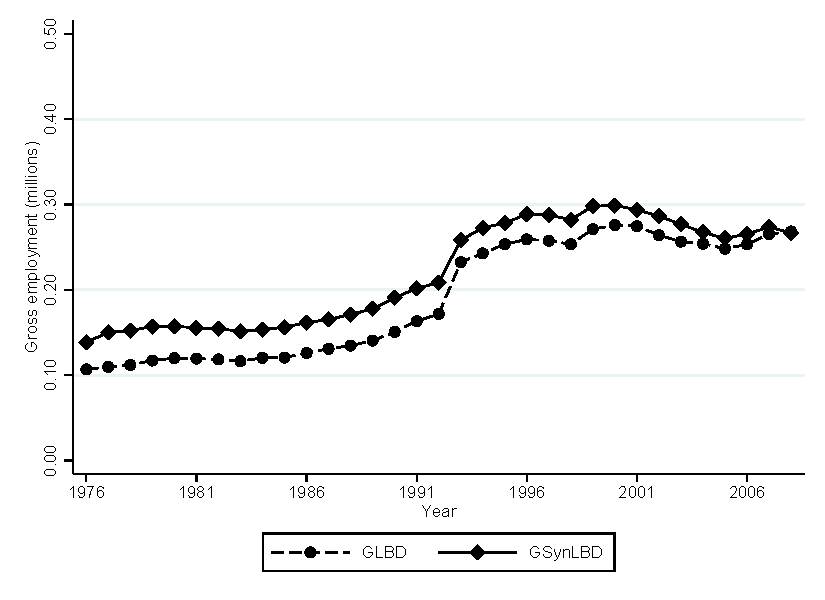
\includegraphics[trim=0 40 0 0,clip,width=\linewidth]{graphs/Gross_employment_level_by_year_bw_GsynLBD.pdf}
%\caption{GSynLBD}
\end{subfigure}\\
\begin{subfigure}[h]{0.48\linewidth}
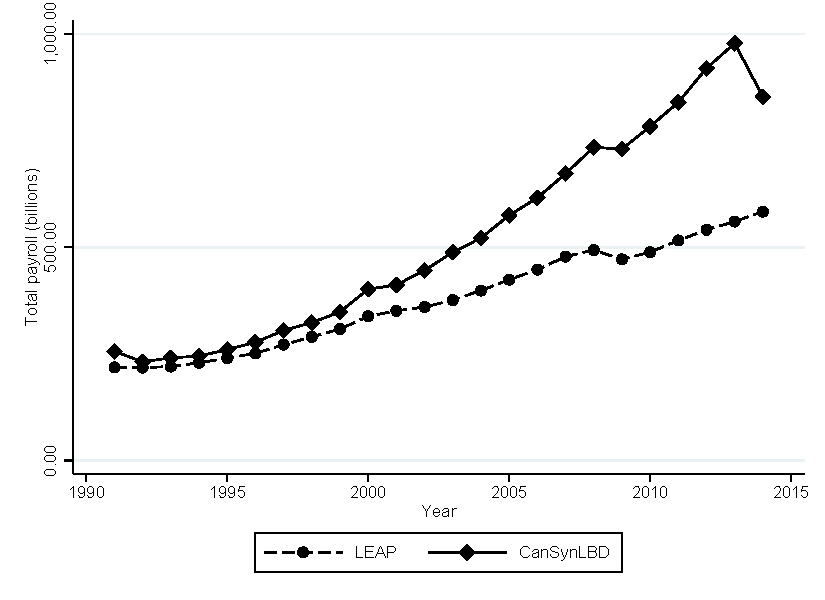
\includegraphics[trim=0 0 0 -20,clip,width=\linewidth]{graphs/Total_payroll_by_year_private_bw.pdf}
\caption{CanSynLBD}
\end{subfigure}
\hfill
\begin{subfigure}[h]{0.48\linewidth}
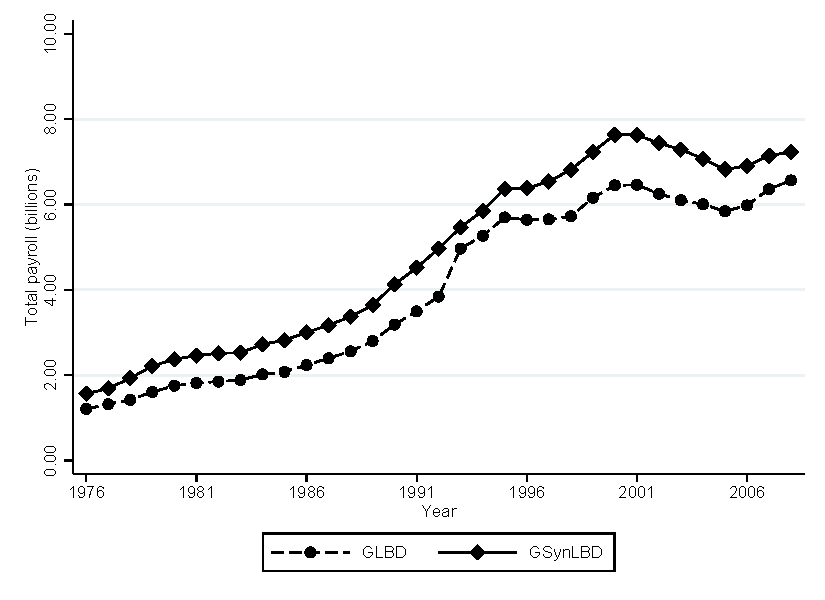
\includegraphics[trim=0 0 0 -20,clip,width=\linewidth]{graphs/Total_payroll_by_year_bw_GsynLBD.pdf}
\caption{GSynLBD}
\end{subfigure}%
\caption{Gross employment level (upper panels) and total payroll (lower panels) by year.}\label{fig:entity_chracteristics}
\end{figure}

Figure \ref{fig:entity_chracteristics} shows a comparison between the synthetic data and the original data for gross employment level (upper panels) and total payroll (lower panels) by year for the Canadian (left panels) and the German (right panels) case. While the general trends are preserved for both data sources, the results for the German synthetic data resemble the trends from the original data more closely. For the Canadian data the positive trends over time are generally overestimated. Looking only at the manufacturing sector in Canada (see Figure \ref{fig:entity_chracteristics_manufac} in the Appendix), we find that the general trends are better preserved. However, the absolute numbers are always underestimated in the synthetic data.
\todo{Move the footnote to an earlier section, in which we describe in general terms, which parts of the data have been synthesized}\footnote{The private sector comprises all industries including the manufacturing sector except the public sector  (NAICS 61, 62, and 91)} 



%\begin{figure} [H]
%\centering
%\label{tab:all:characteristics}
%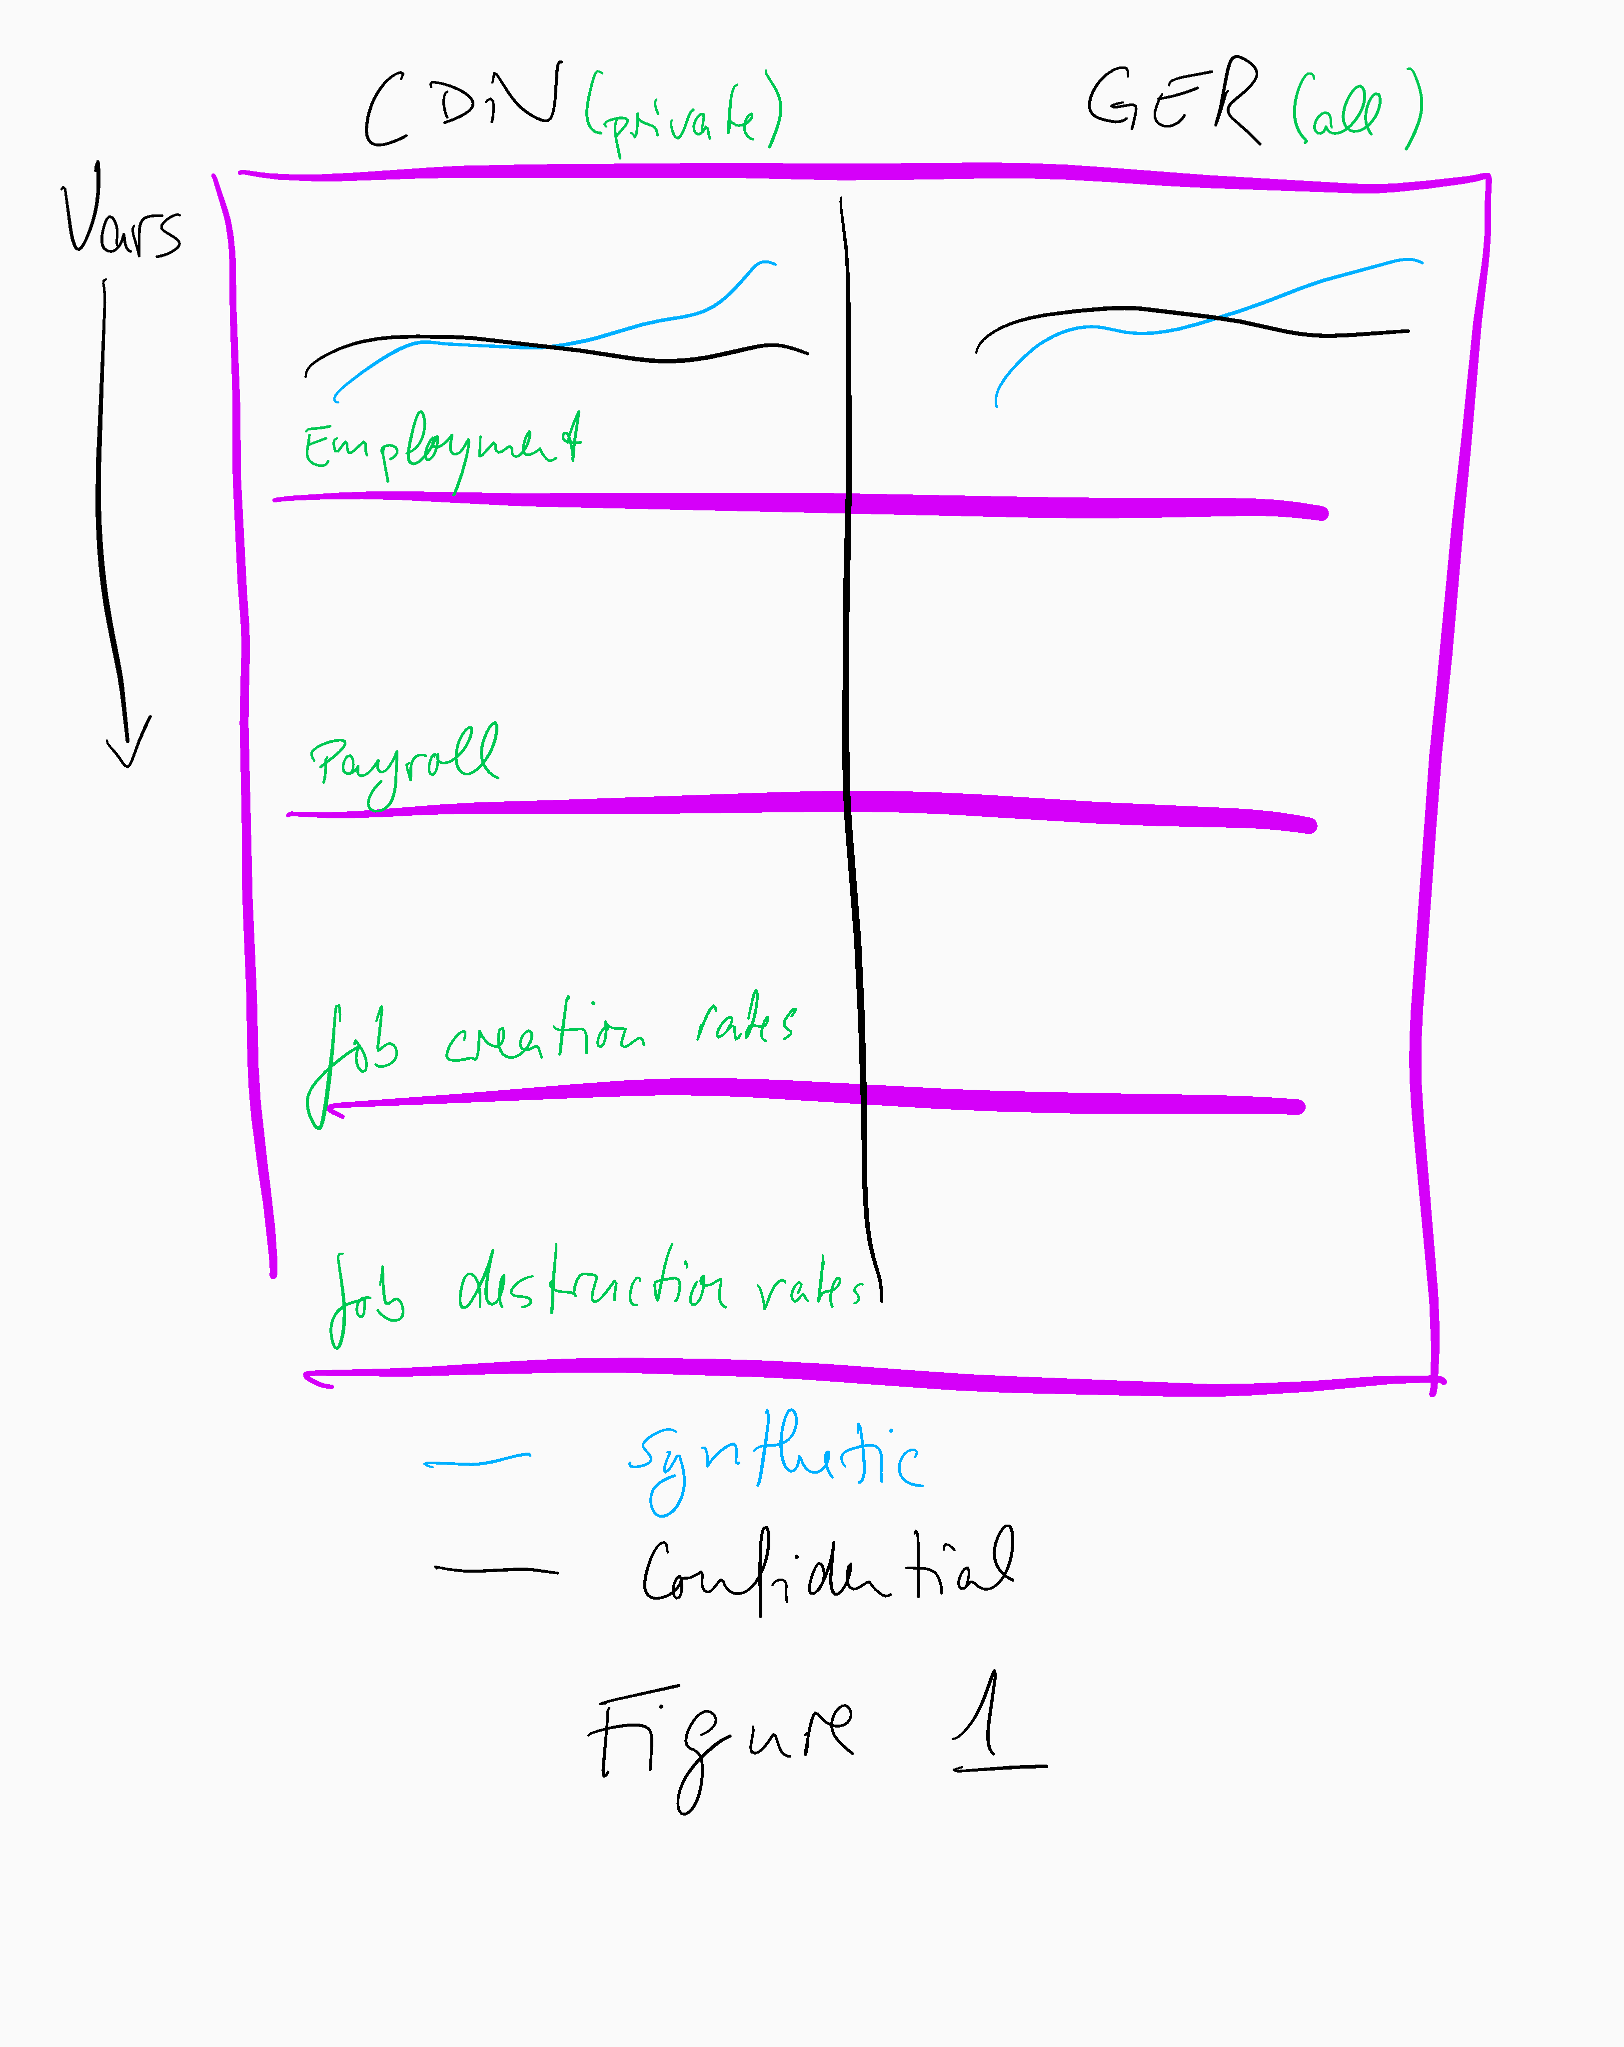
\includegraphics[width=.8\linewidth]{graphs/Figure1-placeholder.png} 
%\caption{Alternate graph} 
%\begin{minipage}{0.48\linewidth}
%{\footnotesize To be computed in R, or redone in Stata using GPH files. \par}
%\end{minipage}
%\end{figure}


\subsection{Dynamics of Job Flows}

\begin{figure}[t]
\begin{subfigure}[h]{0.48\linewidth}
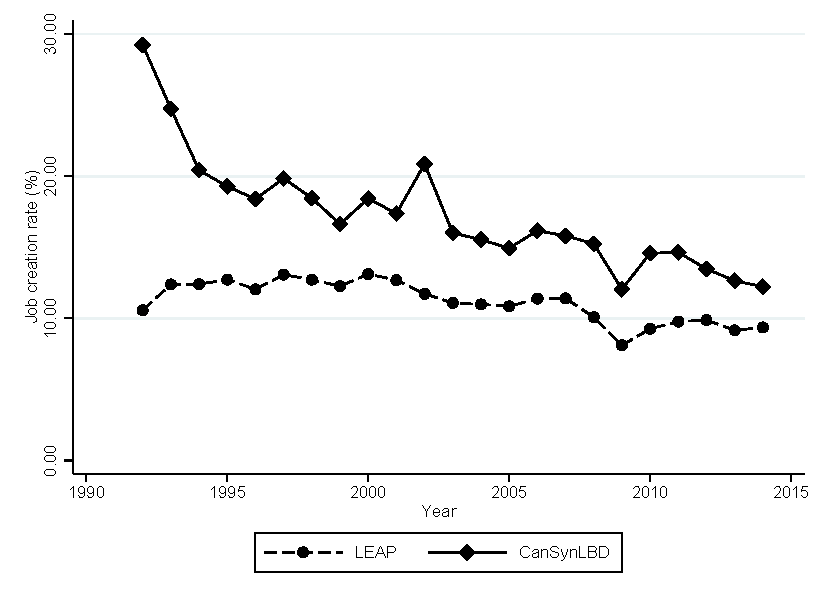
\includegraphics[trim=0 40 0 0,clip, width=\linewidth]{graphs/Job_creation_rate_by_year_private_bw.pdf}
%\caption{CanSynLBD}
\end{subfigure}
\hfill
\begin{subfigure}[h]{0.48\linewidth}
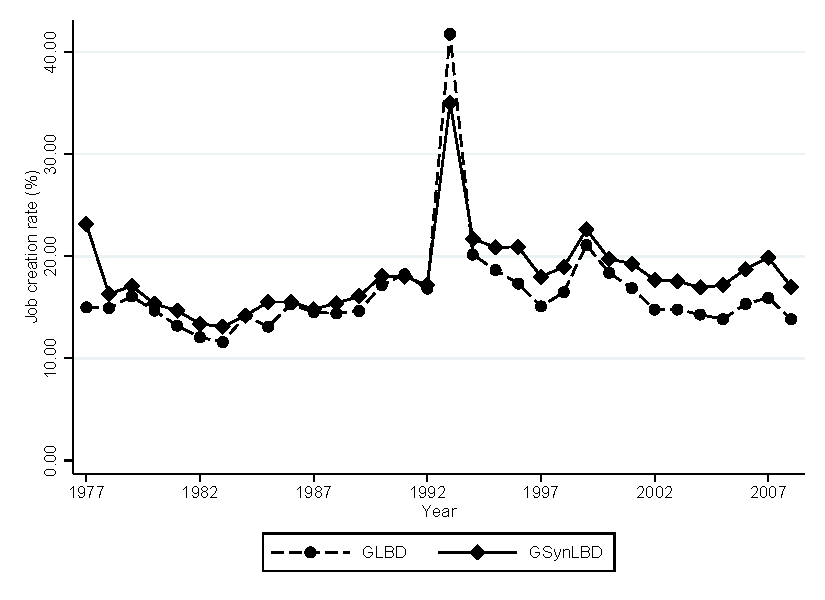
\includegraphics[trim=0 40 0 0,clip,width=\linewidth]{graphs/Job_creation_rate_by_year_bw_GsynLBD.pdf}
%\caption{GSynLBD}
\end{subfigure}\\
\begin{subfigure}[h]{0.48\linewidth}
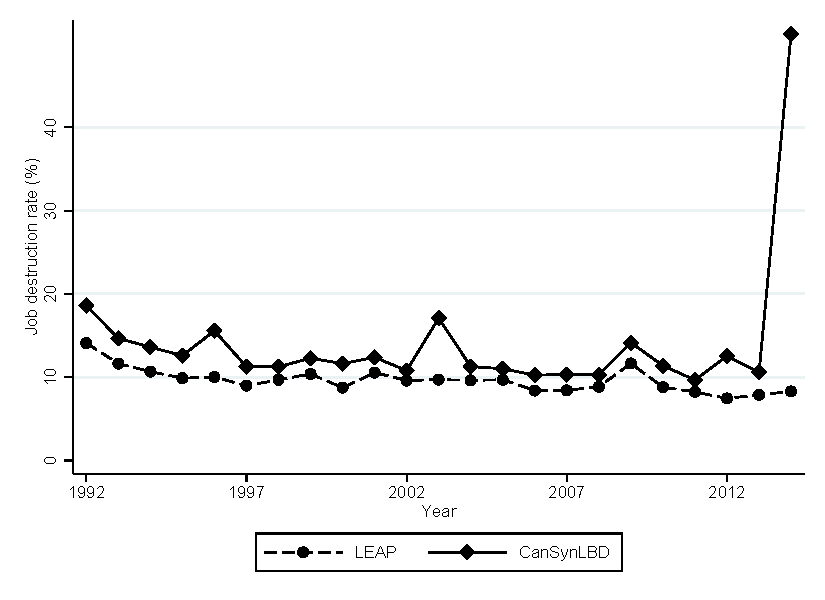
\includegraphics[trim=0 0 0 -20,clip,width=\linewidth]{graphs/Job_destruction_rate_by_year_private_bw.pdf}
\caption{CanSynLBD}
\end{subfigure}
\hfill
\begin{subfigure}[h]{0.48\linewidth}
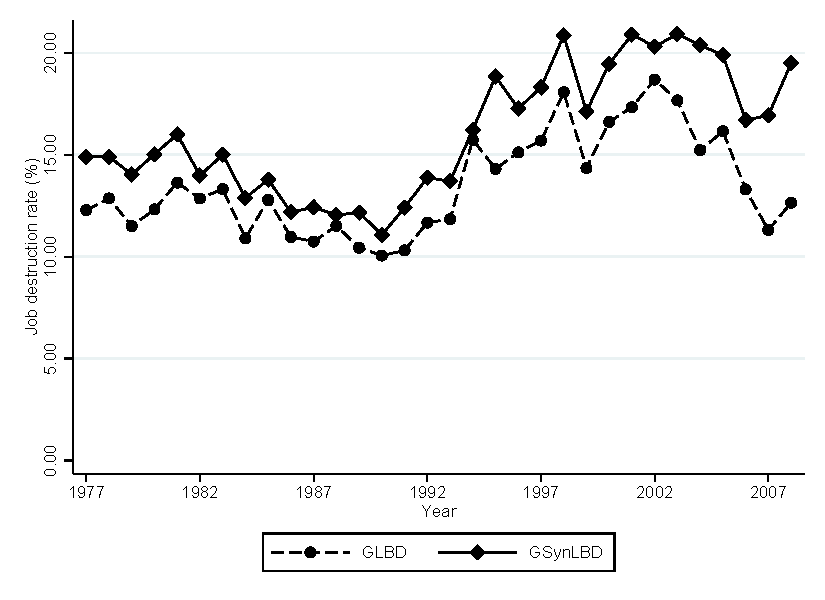
\includegraphics[trim=0 0 0 -20,clip,width=\linewidth]{graphs/Job_destruction_by_year_bw_GsynLBD.pdf}
\caption{GSynLBD}
\end{subfigure}%
\caption{Job creation rates (upper panels) and job destruction rates (lower panels) by year.}\label{fig:job_flows}
\end{figure}

Key statistics commonly computed from business registers such as the LEAP or the BHP include job flows over time. Following \citet{DavisHaltiwangerSchuh}, job creation is defined as the sum of all employment gains from expanding firms from year $t-1$ to year $t$ including entry firms. The job destruction rate is defined as the sum of all employment losses from contracting firms from year $t-1$ to year $t$ including exiting firms. Figure \ref{fig:job_flows} depicts these job creation (upper panels) and destruction rates (lower panels) for the Canadian (left panels) and German case (right panels). The findings are similar to the findings in the previous section. The general patterns are preserved for both data sources, but the the trends align more closely for the German data. Even the substantial increase in job creations in 1993, which can be attributed to the integration of the data from Eastern Germany after reunification, is preserved in the synthetic data. Still, there seems to be a small but systematic overestimation of job creation and destruction rates in both synthetic data sources. The substantial deviation in the job destruction rate in the last year of CanSynLBD is an artefact, which requires further investigation. 
\todo{Is there an explanation for this artefact?}
The results for the manufacturing sector in Canada included in Figure \ref{fig:job_flows_manufac} in the Appendix are comparable to the results for the entire private sector.
\todo{Should we still include the net job creation rate? I would say no.}
%Net job creation is the job creation rate minus the job destruction rate. Figures \ref{JobCreationPrivate} and \ref{JobCreationManufacturing} show the job creation rates from the CanSynLBD compared againg those of the LEAP. These figures show that the manufacturing sector has closer pattern than the private sector. We find a similar patterns for net job creation rates (Panels x and y of Figures \ref{NetJobCreationPrivate} and  \ref{NetJobCreationManufacturing}).




\subsection{Entity Dynamics}

\begin{figure}[t]
\begin{subfigure}[h]{0.48\linewidth}
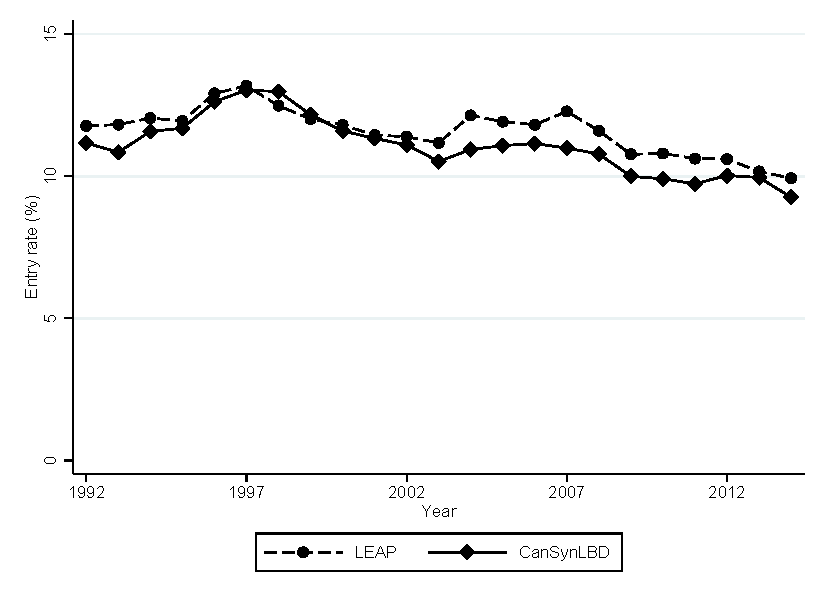
\includegraphics[trim=0 40 0 0,clip, width=\linewidth]{graphs/Entry_rate_bw_private.pdf}
%\caption{CanSynLBD}
\end{subfigure}
\hfill
\begin{subfigure}[h]{0.48\linewidth}
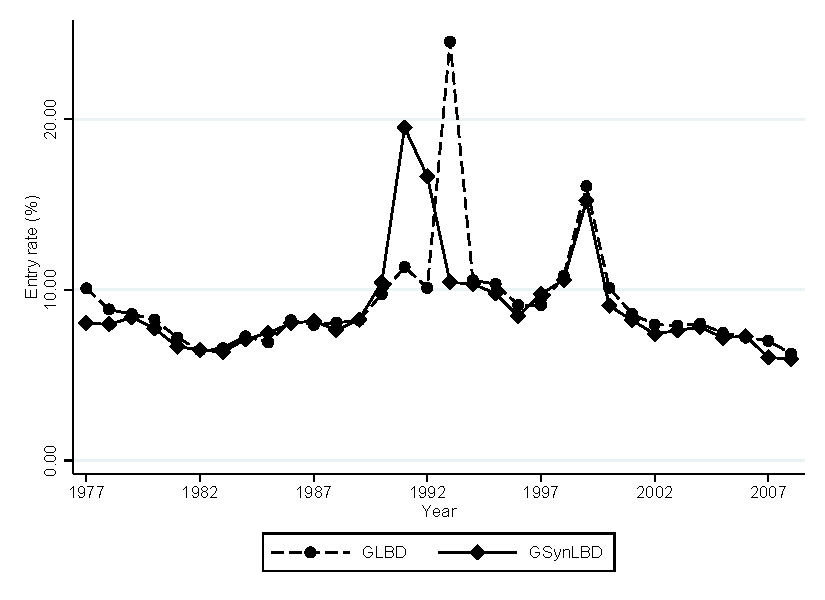
\includegraphics[trim=0 40 0 0,clip,width=\linewidth]{graphs/Entry_rate_bw_GsynLBD.pdf}
%\caption{GSynLBD}
\end{subfigure}\\
\begin{subfigure}[h]{0.48\linewidth}
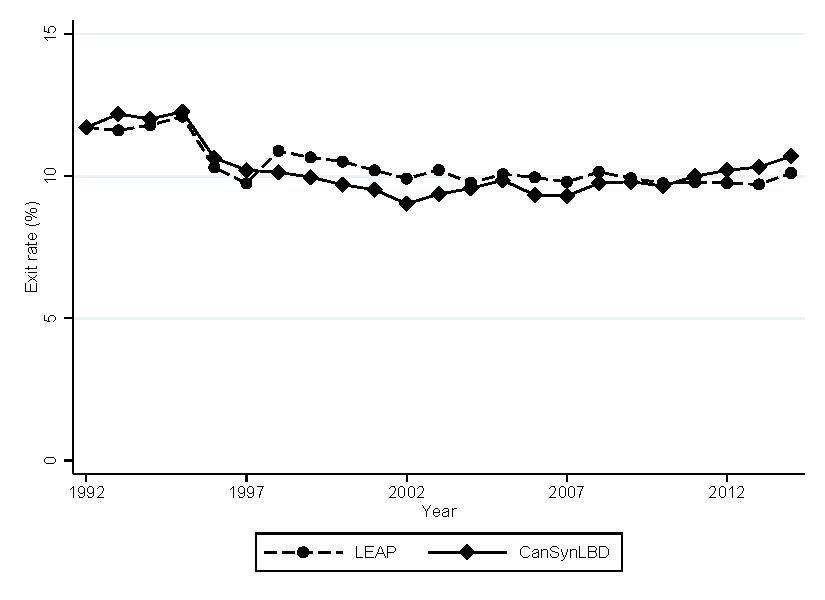
\includegraphics[trim=0 0 0 -20,clip,width=\linewidth]{graphs/Exit_rate_bw_private.pdf}
\caption{CanSynLBD}
\end{subfigure}
\hfill
\begin{subfigure}[h]{0.48\linewidth}
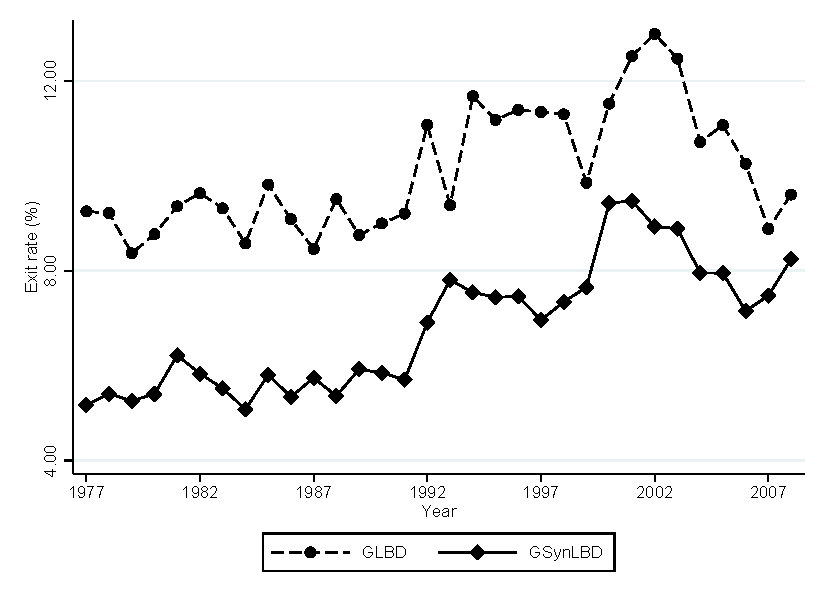
\includegraphics[trim=0 0 0 -20,clip,width=\linewidth]{graphs/Exit_rate_bw_GsynLBD.pdf}
\caption{GSynLBD}
\end{subfigure}
\caption{Entry rates (upper panels) and exit rates (lower panels) by year.}\label{fig:FirmDynamics}
\end{figure}

To assess how well the synthetic data capture entity dynamics, we also compute entry and exit rates, i.e. how many new entities appear in the data and how many cease to exist relative to the population of entities in a specific year. Figure \ref{fig:FirmDynamics} shows that those rates are very well preserved for both data sources. Only the re-unification spike in the entry rates in the German data is not preserved correctly. While the original data show a large spike in entry rates for 1993, because this was the year when detailed information about Eastern German establishments was integrated for the first time, the synthetic data shows increased entry rates in the two previous years. We speculate that this occurs as the establishments were successively integrated into the data starting in 1991, but for many of them no information regarding payroll and number of employees was reported in the first two years. Thus, they exist in the original data, but the establishment size is reported as missing. Such a combination is not possible in the synthetic data. Whenever an establishment exists, it has to have a positive number of employees. Since entry rates are computed by looking at whether the establishment information changed from missing to a positive value, most of the Eastern German establishments only exist from 1993 on-wards in the original data, but from 1991 in the synthetic data.
The second spike in the entry rate in the German data in 1999 occurs, as marginally employed had to be reported for the first time in this year. Thus, all establishments that only have marginally employed employees are also included in the BHP from 1999 on-wards.
%To show further those rates are similar, we compute the divergence of entry rate as the entry rate of CanSynLBD net the entry rate of LEAP as well as the divergence of exit rate as the exit rate of CanSynLBD net the exit rate of LEAP (see Figure \ref{Divergence}).





\subsection{Distribution of variables across time and industry}

The synthesis code for the synLBD ensures that the total number of entities that ever exist within the considered time frame  match exactly between the original data and the synthetic data. But because each entity's entry and exit date are synthesized, the total number of entities at a particular point in time may differ, and with it employment and payroll. To investigate, how well the information is preserved at any given point in time, we compute the following statistic:
\begin{equation}
    \label{eq:share_employment}
x_{its} = X_{its}/\sum_{i} \sum_{t} X_{its}, 
\end{equation}
where $i$ is the index for the industry (aggregated to the two digit level for the Canadian data), $t$ is the index for the year and $s$ denotes the data source (original or synthetic). $X_{its}=\sum_j X_{itsj}, j=1,\ldots,n_{it}$ is the variable of interest aggregated at the industry level and $n_{it}$ is the number of entities in industry $i$ at time point $t$. For example $X_{its}$ could be the total payroll in 1999 for a specific industry in the original data. To compute the statistic provided in Equation (\ref{eq:share_employment}), this number is then divided by the total payroll aggregated across all industries and years.
Figure \ref{fig:FirmShare} plots the results from the original data against the results from the synthetic data for the variables \textit{number of entities}, \textit{employment}, and \textit{payroll}. If the information is well preserved, all points should be close to the 45 degree line. 

We find that the share of entities is well preserved for both data sources, but share of employment and share of payroll vary more in the Canadian data with an upward bias for the larger shares. Of course, it should be noted that the German data are only aggregated over two industries whereas the Canadian data contains XX\todo{do we have this number?} different industry codes on the two digit level. This implies that the results for the Canadian data evaluate the utility at a much more detailed level and thus lower analytical validity compared to the German results is to be expected. The results for Canada improve, when looking only at the manufacturing sector (see Figure \ref{fig:FirmShare_manufac} in the Appendix).

%We inspect this distribution in the Canadian data, by industry, in the following figures.\footnote{Since the German data was only generated for a very small number of industries, we skip this step for Germany.} 


%Figures~\ref{FirmSharePrivate} and \ref{FirmShareManufacturing} plot the share of firms by two-digit industry and year for both the Canadian synthetic  and confidential data. If only contemporaneous features (employment, payroll), and birth and death of the synthetic entities were the same, all observations would be on the 45 degree line. The figures show some divergence of the within-industry distribution across time. 


%Given a distribution of entities alive, we can also compute the share of observed characteristics across time and industry. Shares of a variable $X$ are computed as a fraction of the sum of $X$ across \textit{all} years and industries:

%\begin{equation}
%    \label{eq:share_employment}
%x_{its} = X_{its}/\sum_{i} \sum_{t} X_{its}, 
%\end{equation}

%where $i$ are two-digit industries, $t$ are  years in-sample, $s$ indicates whether it is in the synthetic or confidential data, and $X_{its}$ is the sum of the variable of interest $X$ for industry $i$ and year $t$ in  dataset $s$.

\begin{figure}
\begin{subfigure}[h]{0.48\linewidth}
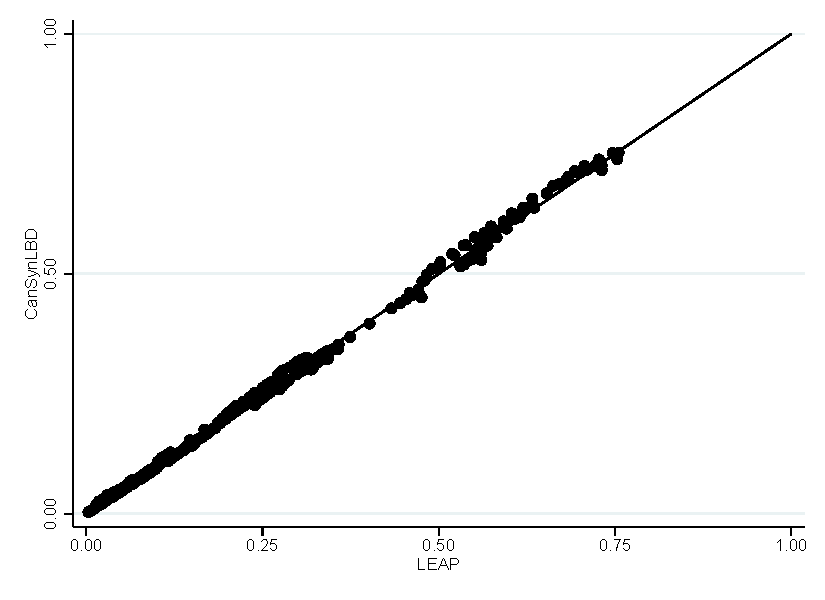
\includegraphics[trim=0 10 0 0,clip, width=\linewidth]{graphs/Share_of_firms_by_NAICS_two-digit_and_year_private_bw.pdf}
%\caption{CanSynLBD}
\end{subfigure}[t]
\hfill
\begin{subfigure}[h]{0.48\linewidth}
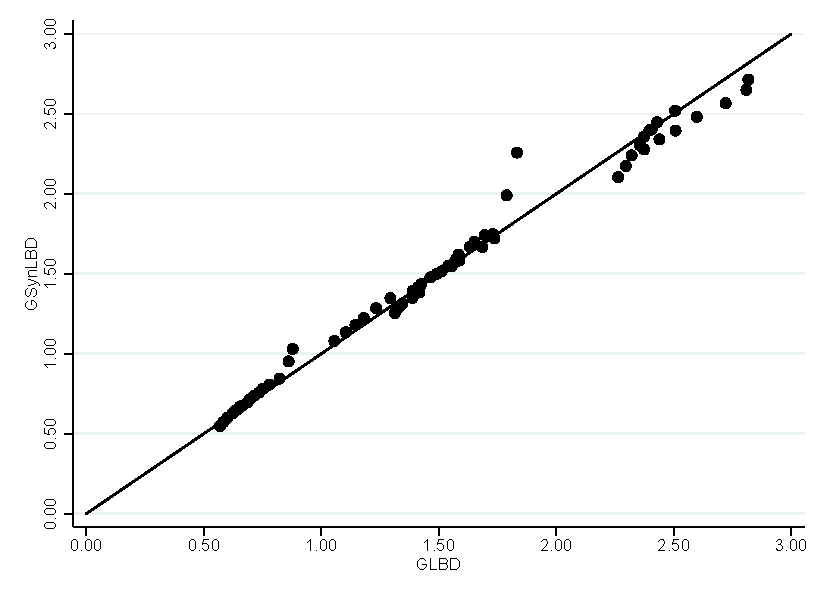
\includegraphics[trim=0 10 0 0,clip,width=\linewidth]{graphs/Share_of_firms_by_NAICS_and_year_bw_GsynLBD.pdf}
%\caption{GSynLBD}
\end{subfigure}\\
\begin{subfigure}[h]{0.48\linewidth}
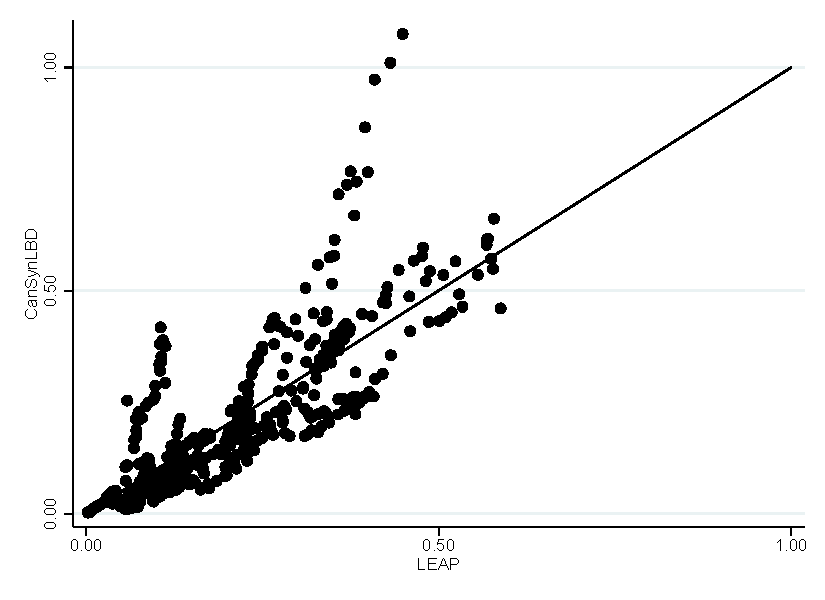
\includegraphics[trim=0 10 0 -20,clip,width=\linewidth]{graphs/Share_of_employment_by_NAICS_two-digit_and_year_private_bw.pdf}
%\caption{CanSynLBD}
\end{subfigure}
\hfill
\begin{subfigure}[h]{0.48\linewidth}
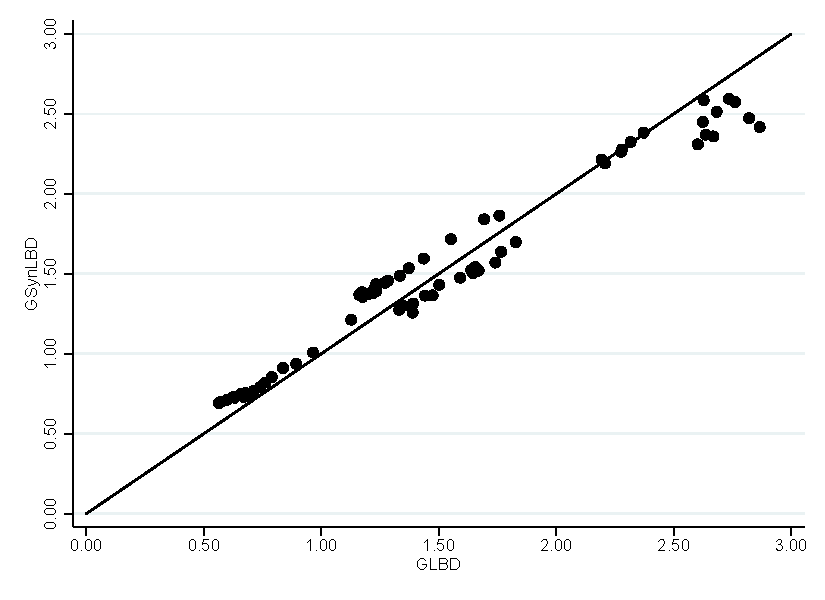
\includegraphics[trim=0 10 0 -20,clip,width=\linewidth]{graphs/Share_of_employment_by_NAICS_and_year_bw_GsynLBD.pdf}
%\caption{GSynLBD}
\end{subfigure}\\
\begin{subfigure}[h]{0.48\linewidth}
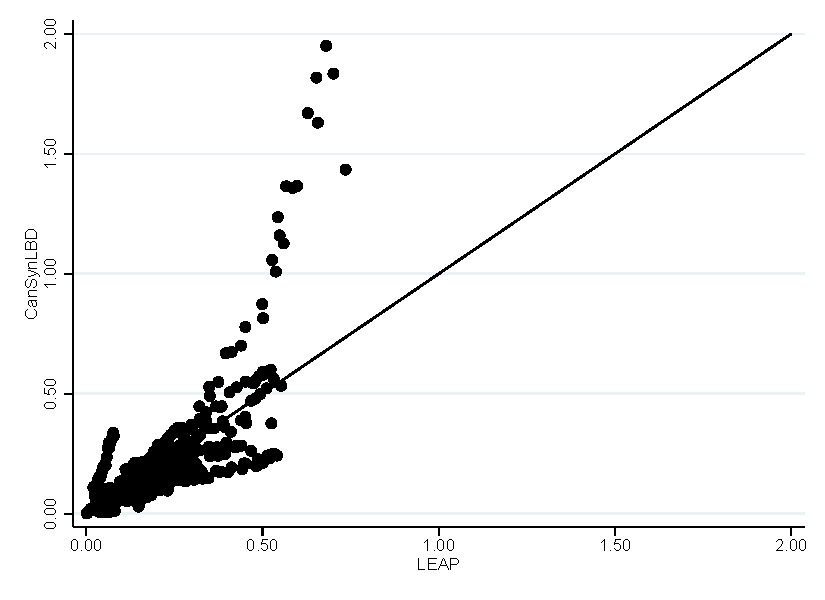
\includegraphics[trim=0 0 0 -20,clip,width=\linewidth]{graphs/Share_of_payroll_by_NAICS_two-digit_and_year_private_bw.pdf}
\caption{CanSynLBD}
\end{subfigure}
\hfill
\begin{subfigure}[h]{0.48\linewidth}
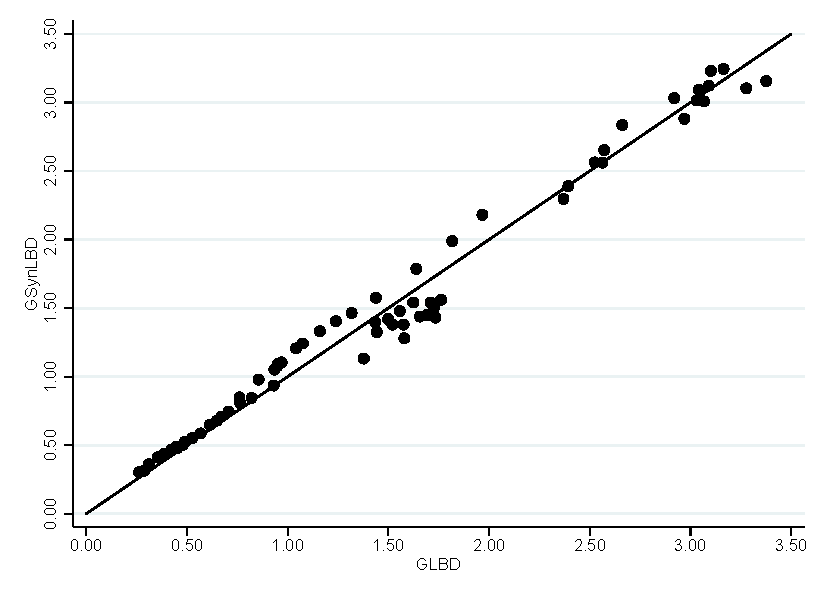
\includegraphics[trim=0 0 0 -20,clip,width=\linewidth]{graphs/Share_of_payroll_by_NAICS_and_year_bw_GsynLBD.pdf}
\caption{GSynLBD}
\end{subfigure}%
\caption{Share of entities (upper panels), share of employment (middle panels), and share of payroll (lower panels) by year and industry.}\label{fig:FirmShare}
\end{figure}

%\begin{figure} [H]
%\centering
%\label{tab:Can:FirmDynamics}
%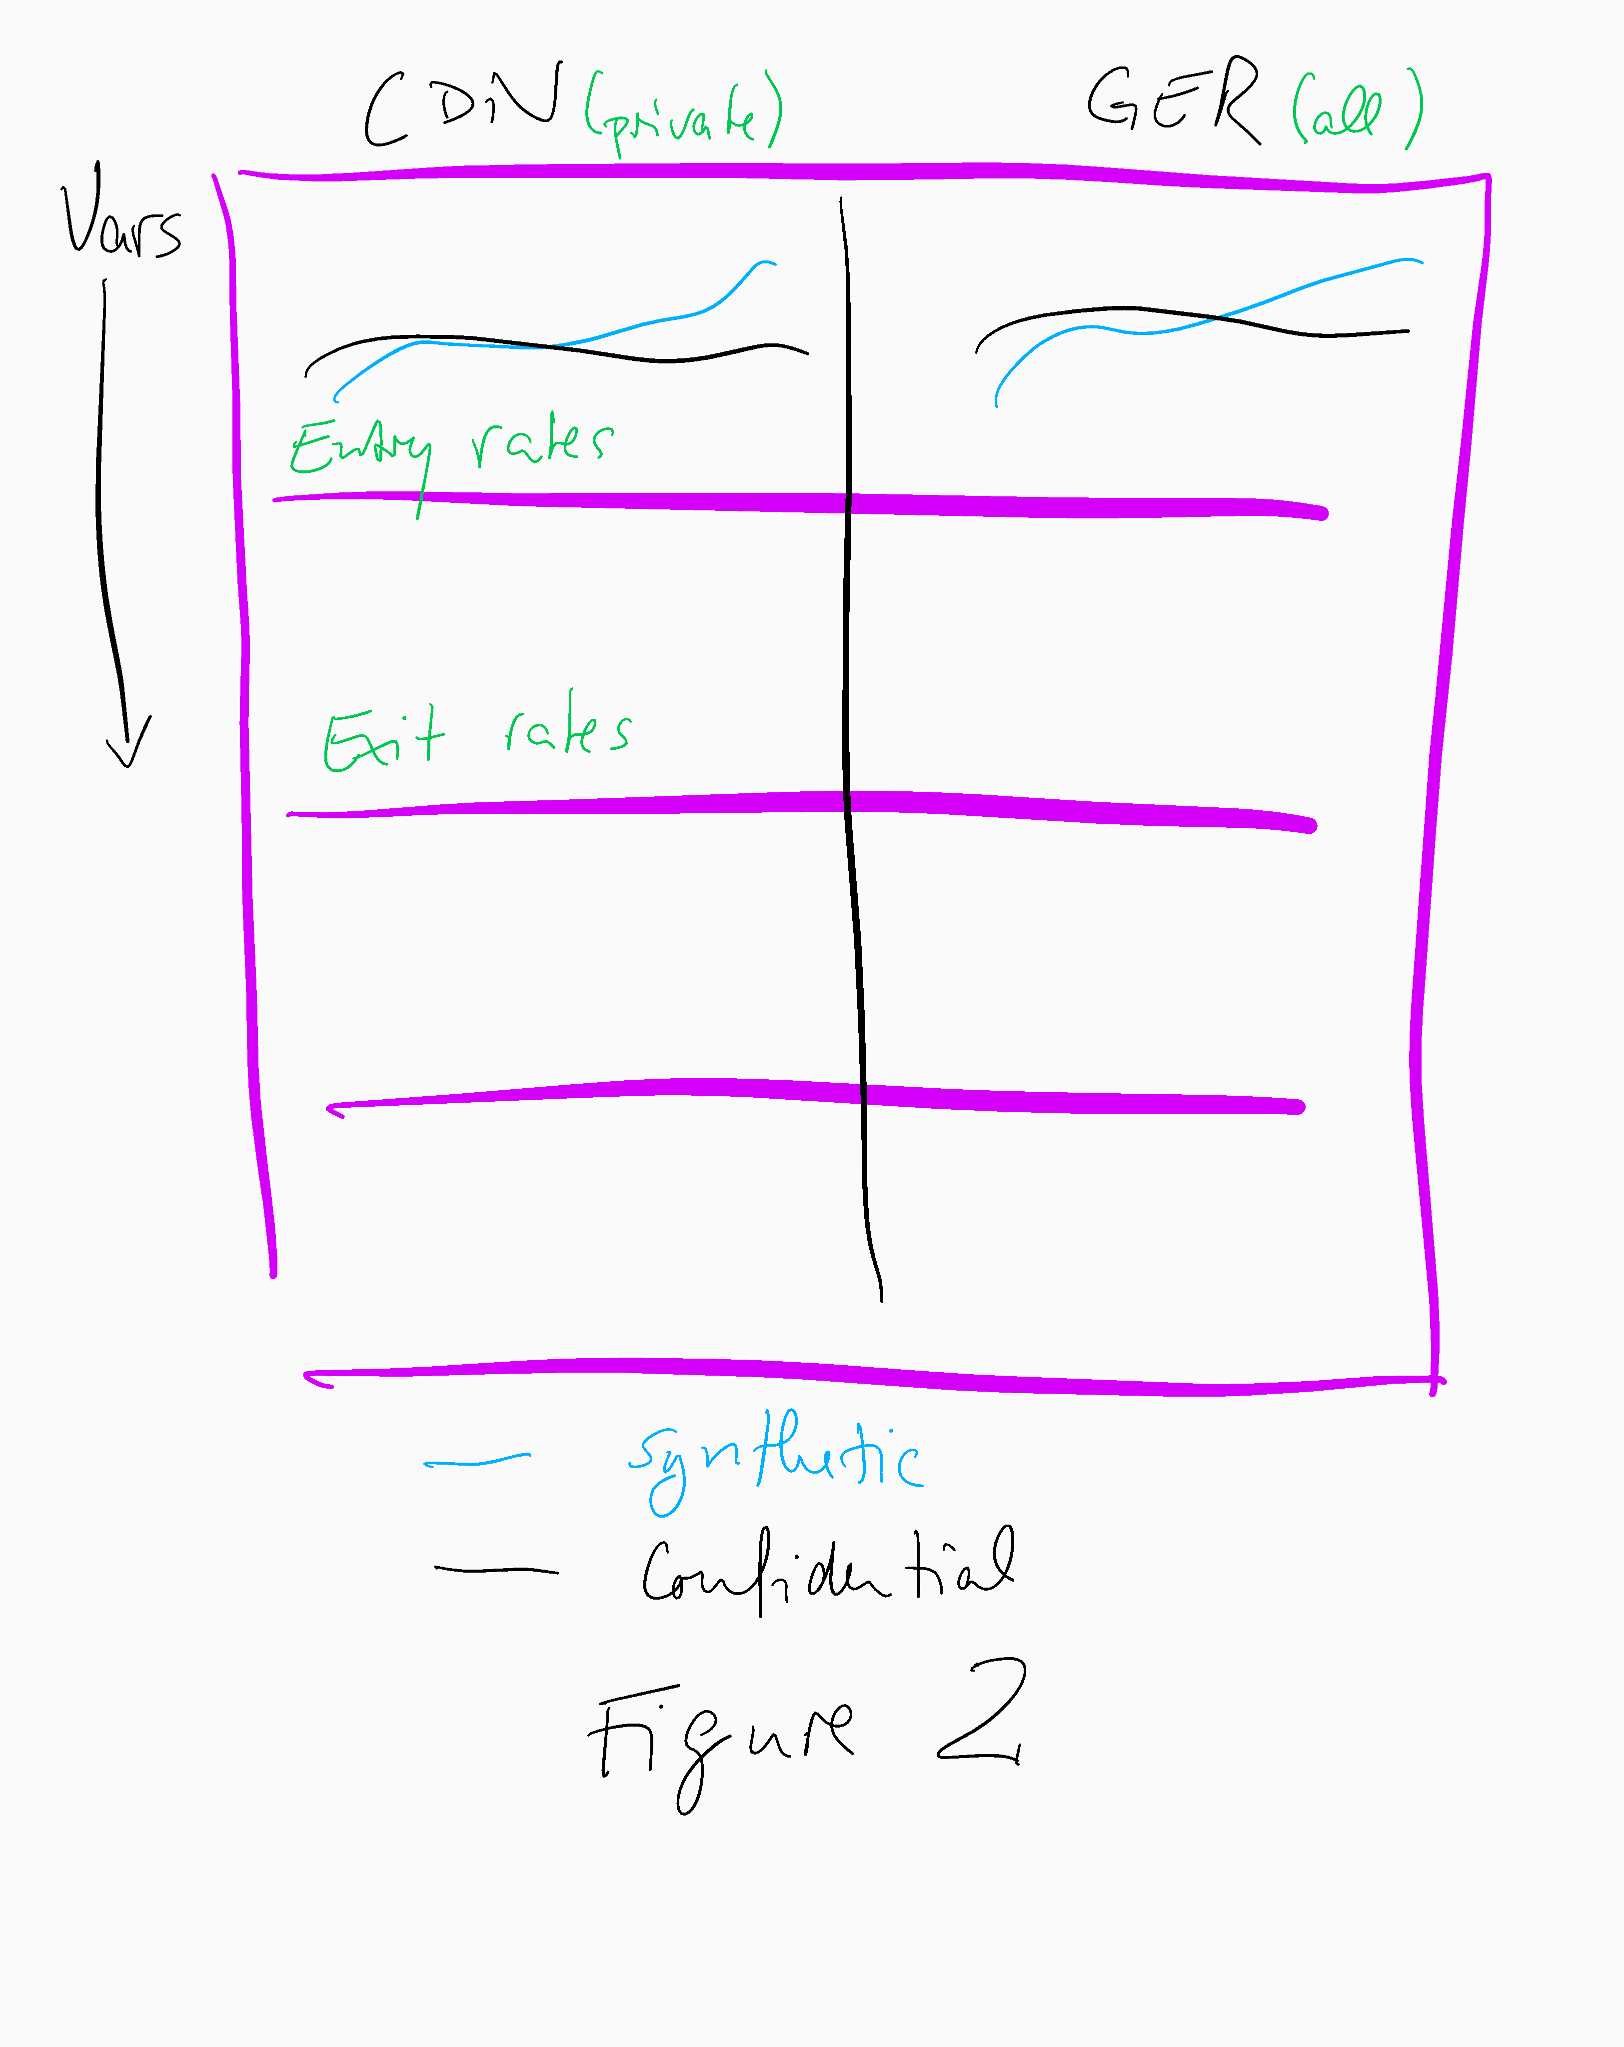
\includegraphics[width=.8\linewidth]{graphs/Figure2-placeholder.png} 
%\caption{Alternate graph} 
%\begin{minipage}{0.48\linewidth}
%{\footnotesize To be computed in R, or redone in Stata using %GPH files. Detailed data are in the appendix. \par}
%\end{minipage}
%\end{figure}

%\todo{Also consolidate graphs here}
%\%begin{figure} [H]
%\centering
%\label{tab:all:shares}
%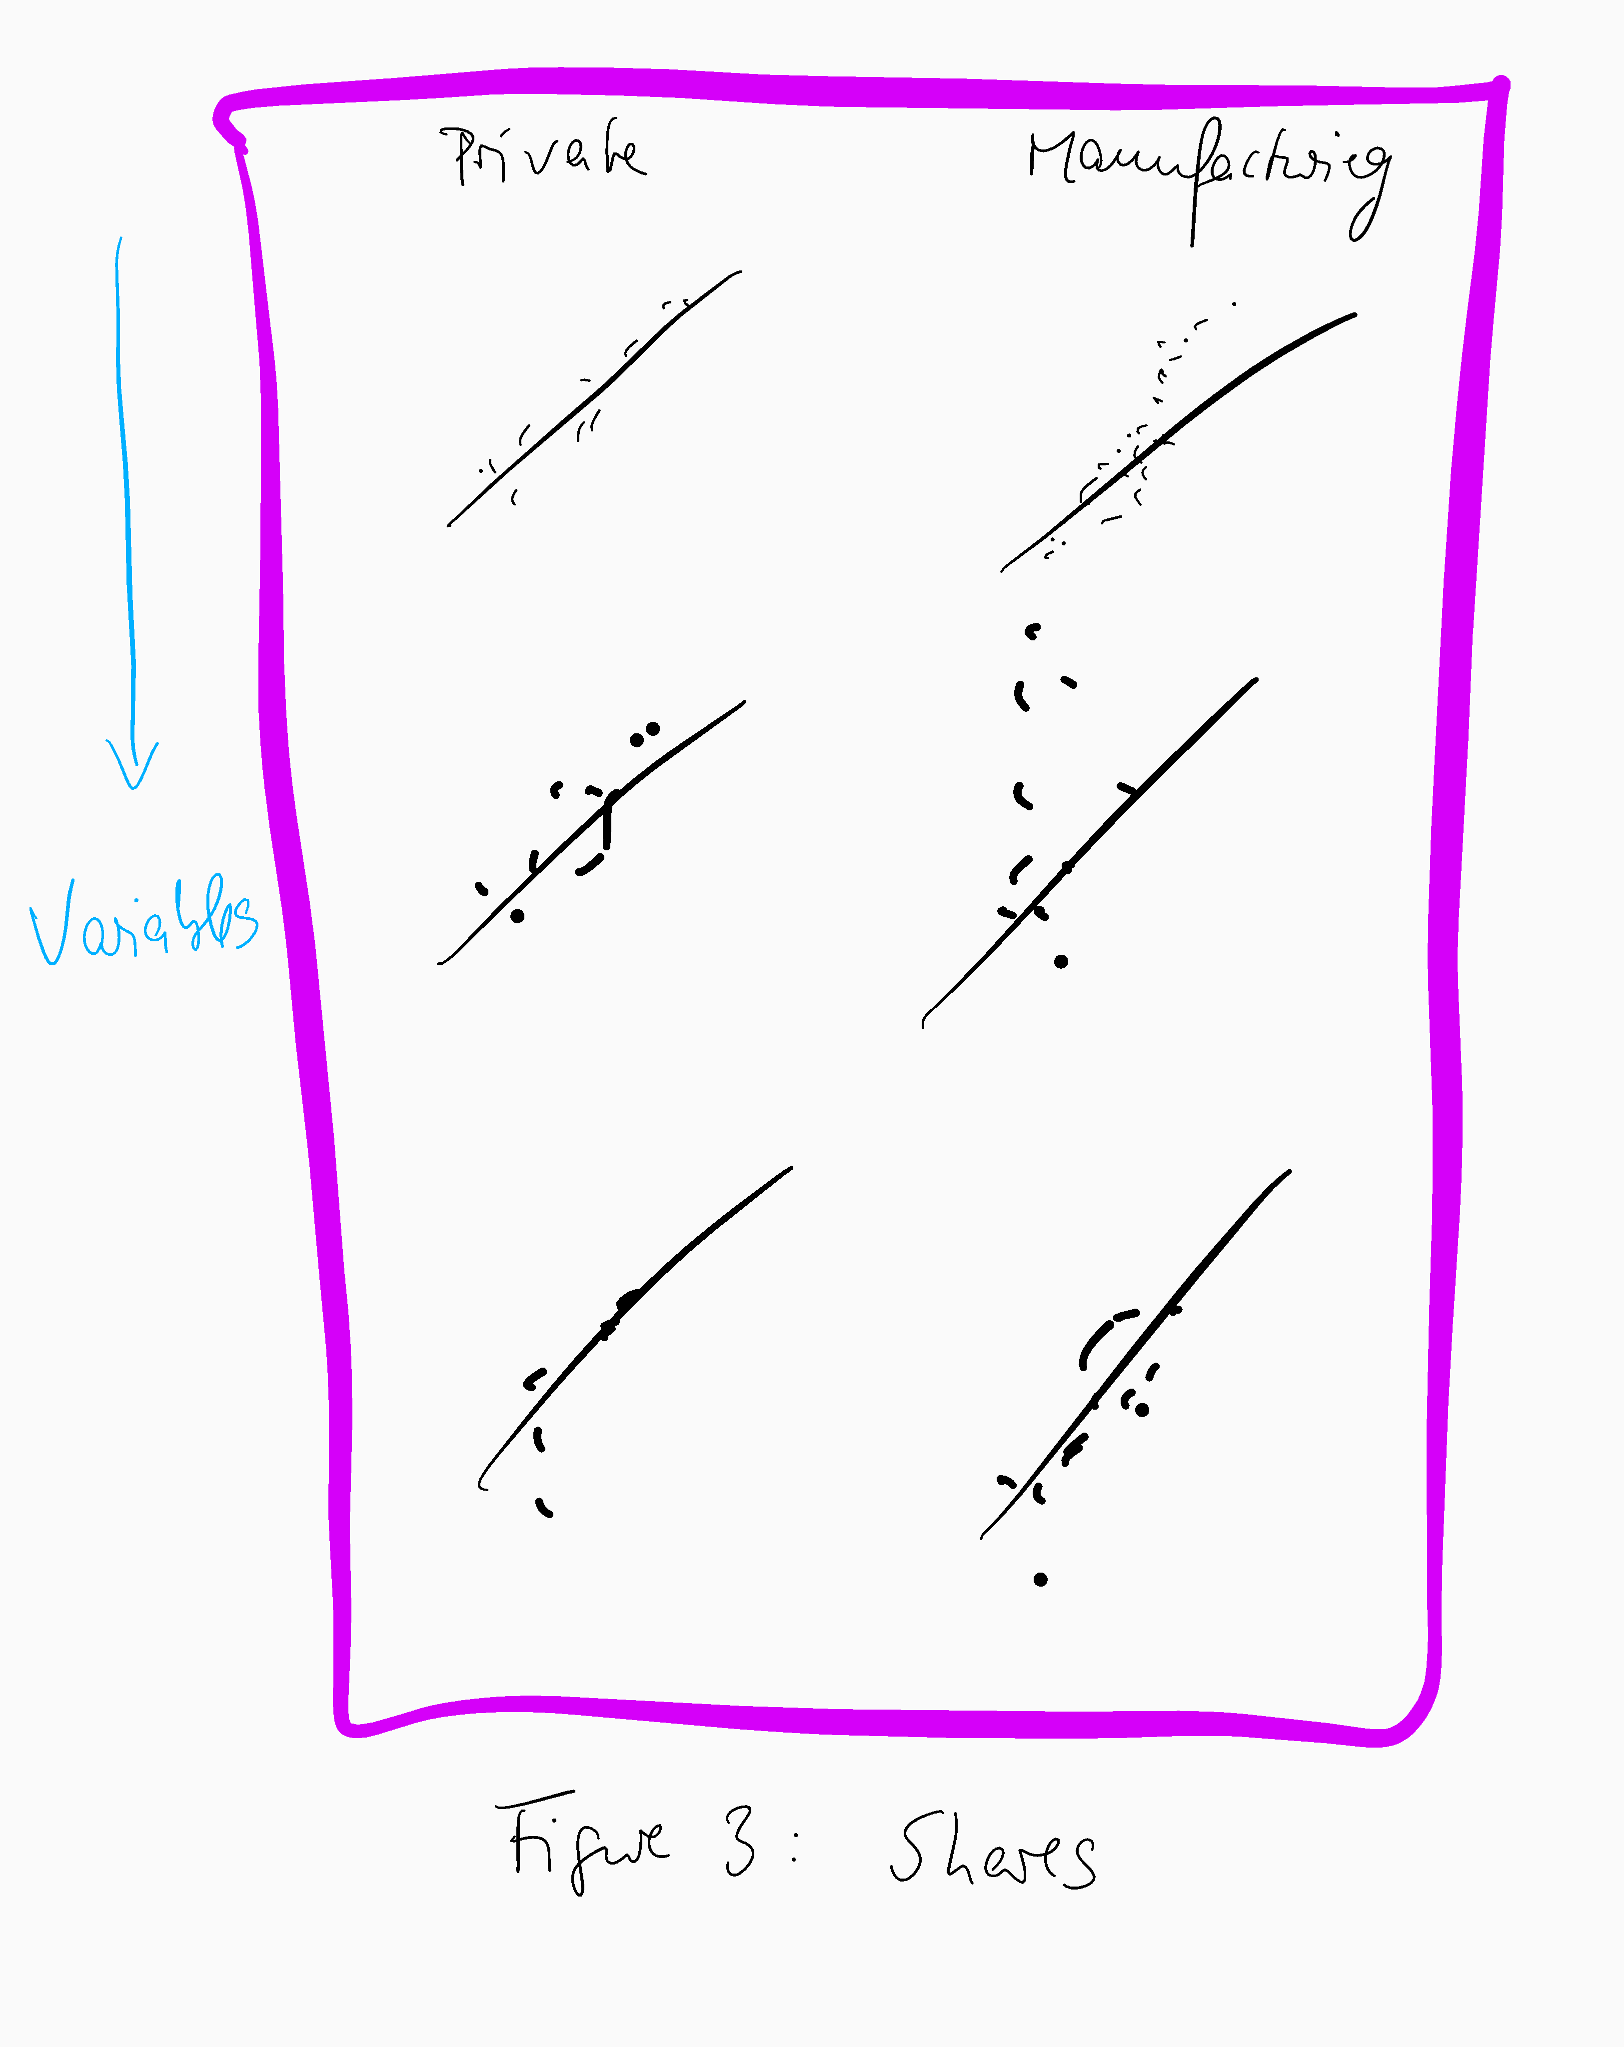
\includegraphics[width=.8\linewidth]{graphs/Figure3-placeholder.png} 
%\caption{Alternate graph} 
%\begin{minipage}{0.48\linewidth}
%{\footnotesize To be computed in R, or redone in Stata using GPH files. Detailed data are in the appendix. \par}
%\end{minipage}
%\end{figure}


%Figures~\ref{EmploymentSharePrivate} and \ref{EmploymentShareManufacturing} plot the share of employment by two-digit industry and year for both  CanSynLBD and the LEAP database. 
%Employment shares  do not cluster along the 45-degree line. However, this hides significant differences between sectors. For instance,  the share of employment for the manufacturing sector does show stronger clustering along the 45-degree line.


%Figures~\ref{PayrollSharePrivate} and~\ref{PayrollShareManufacturing} plot the share of \textit{payroll} by two-digit industry and year for both CanSynLBD and LEAP database. In general, shares do not cluster along the 45-degree line, though a focus on  the manufacturing sector again shows stronger clustering along the 45-degree line.


\subsection{pMSE}


% Table created by stargazer v.5.2.2 by Marek Hlavac, Harvard University. E-mail: hlavac at fas.harvard.edu
% Date and time: Fri, Feb 14, 2020 - 06:10:27 PM
\begin{table}[!htbp] \centering 
  \caption{pMSE by sector and country} 
  \label{tab:pmse} 
\begin{tabular}{@{\extracolsep{5pt}} ccccc} 
\\[-1.8ex]\hline 
\hline \\[-1.8ex] 
country & sector & pMSE & pMSE.ratio & pMSE.standardized \\ 
\hline \\[-1.8ex] 
Canada & Manufacturing & 0.0041 & 9196.35 & 18390.69 \\ 
Canada & Private & 0.0121 & 419128.55 & 838255.1 \\ 
Germany & Universe & 0.0013 & 595.05 & 2623.24 \\ 
\hline \\[-1.8ex] 
\end{tabular} 
\end{table} 


To compute the $pMSE$, we estimate Equation (\ref{pMSE}) using logit models. The estimated $pMSE$ is 0.0121 for the Canadian data (0.0041 when looking only at the manufacturing sector) and 0.0013 for the German data (see Table~\ref{tab:pmse}). While these numbers may seem small, \citet{Snoke_RSSA2018} provide an appropriate expected value, and Table~\ref{tab:pmse} reports quite large numbers, suggesting that the synthetic data do not have very high analytical validity.

%These numbers are difficult to interpret on an absolute scale, but the fact that they are all close to zero seems to imply that the measure indicates a high level of analytical validity. However, as pointed out by \citet{Woo_Reiter_Oganian_Karr_2009}, the value of the $pMSE$ depends on the model specification of the propensity score model. Including more predictors or interaction terms in the model will typically lead to an increase in the $pMSE$. This was also confirmed by \citet{Snoke_RSSA2018}, who showed that under the assumption that both datasets come from the same data generating process, the expected value of the $pMSE$ is $(k-1)(1-c)^2c/N$, where $k$ is the number of parameters included in the propensity model, $c$ is the proportion of synthetic records in the stacked dataset and $N$ is the number of records in the stacked dataset. Thus, adding complexity to the propensity score model will generally lead to an increase in the $pMSE$ even if the synthesis model is perfect. The findings of \citet{Snoke_RSSA2018} also illustrate that it is not meaningful to compare the $pMSE$ from the Canadian data to the $pMSE$ from the German data or to the $pMSE$ of the manufacturing sector as the sizes of the datasets are substantially different. 
%=NTTable~\ref{tab:pMSE_regression} shows the results from the estimation of $pMSE$ for the Canadian data.
%\todo{BD: Are those coefficients or marginal effects? Does it make sense to show coefficients? Or are we interested only in the last row? If we are interested in the coefficient, why is there no discussion of those?} 
%\todo{Those are coefficients. I think we are interested in the last row.} 
%$pMSE$ is closer to zero for the manufacturing sector than the private sector in both regressions, consistent with our earlier observations for Canada.

%\newpage

%DISCUSSION IS STILL MISSING.\todo{pMSE discussion}

\subsection{Regression Analysis}

\todo{Need to expand the regression discussion: only one generic model, many others possible, reference to the Singapore presentation by Lars}
To assess how well the synthetic data perform in a more complex model, we estimate a dynamic panel data model for the evolution of employment, using four variants suggested by the economics literature. 
These allow us to assess whether the synthetic data capture variability in economic growth due to industry and firm age - the key variables in the data. 

The base variant is an OLS specification:

\begin{eqnarray}	
\label{eq:OLS}
Emp_{et} & = & \beta_0 + \theta Emp_{e,t-1} + \lambda Pay_{et} + Age_{et}^{T}\beta + \lambda_t + \alpha_i + \epsilon_{et}
\end{eqnarray}
where $Emp_{et}$ is log employment of entity $e$ in year $t$, $Emp_{e,t-1}$ is its one year lag, $Pay_{et}$ is the logarithm of payroll of entity $e$ in year $t$, $Age_{et}$ is a vector of dummy variables for age of entity $e$ in year $t$, $\lambda_t$ is the year fixed effect, $\alpha_i$ is an unobserved time-invariant industry-specific effect, and $\epsilon_{et}$ is the disturbance term of entity $e$ in year $t$. 


As $Emp_{e,t-1}$ is correlated with $\alpha_{i}$ because $Emp_{e,t-1}$ is a function of $\alpha_{i}$, \todo{This may need to be explained for non-economists - why is lagged employment of firm e a function of industry effect alpha i?}
OLS estimators are biased and inconsistent. 
To take this endogeneity bias into account,  \textcite{RePEc:oup:restud:v:58:y:1991:i:2:p:277-297.} suggest a generalized method of moments (GMM) method, and tests to assess the  validity of the model.  To test for autocorrelation, we compute the  $m2$ test  for zero autocorrelation in the  first-differenced errors of order two. The Sargan test is used to verify the validity of instrument subsets. Both tests are computed for each country and industry.

We furthermore estimate the model using the system GMM  method proposed by \textcite{RePEc:eee:econom:v:68:y:1995:i:1:p:29-51} and \textcite{RePEc:eee:econom:v:87:y:1998:i:1:p:115-143}, as well as a variant specifying a first-order moving average using appropriate instruments for both level and difference equation  \parencite{RePEc:eee:econom:v:68:y:1995:i:1:p:29-51,RePEc:eee:econom:v:87:y:1998:i:1:p:115-143}:

\todo{@ JA: $\alpha$ is used twice - not clear - please verify - I have added subscripts}
\begin{eqnarray}	
Emp_{et}&=&\beta_{0,e} +\theta Emp_{e,t-1}+\lambda Pay_{et}+Age_{et}^{T}\beta+\lambda_t+\alpha_i+\epsilon_{et}+\gamma\epsilon_{e,t-1}
\end{eqnarray}


We estimate the model separately on confidential and synthetic data for the private sector (and for Canada, for the manufacturing sector). The estimation results are reported in the Appendix. Generally, we find that the estimated coefficients are different, though of the same sign. Only a small number of models show coefficients that are similar (with a positive confidence interval overlap $J_{k,m}$). The key coefficients - lagged employment and pay - are never close. The mean and median $J_{k,m}$ are negative for all models (Table~\ref{tab:jkm}).



, We find that the CansynLBD data provides similar predictions to LEAP data (Tables  \ref{OLS}).\todo{compute overlap interval} \todo{JA: @Lars, I think you mentioned once that you would like to calculate this. I could calculate using the method explained in the appendix.}

%(Table \ref{Dynamic - GMM}).
% and find similar predictions as before (detailed results in Table~\ref{Dynamic - system GMM}). 

%Table~\ref{Dynamic - system GMM with MA(1)} shows that the CansynLBD provides similar predictions to the LEAP.

\todo{Also consolidate graphs here}
\begin{figure} [H]
\centering
\label{tab:all:estimates}
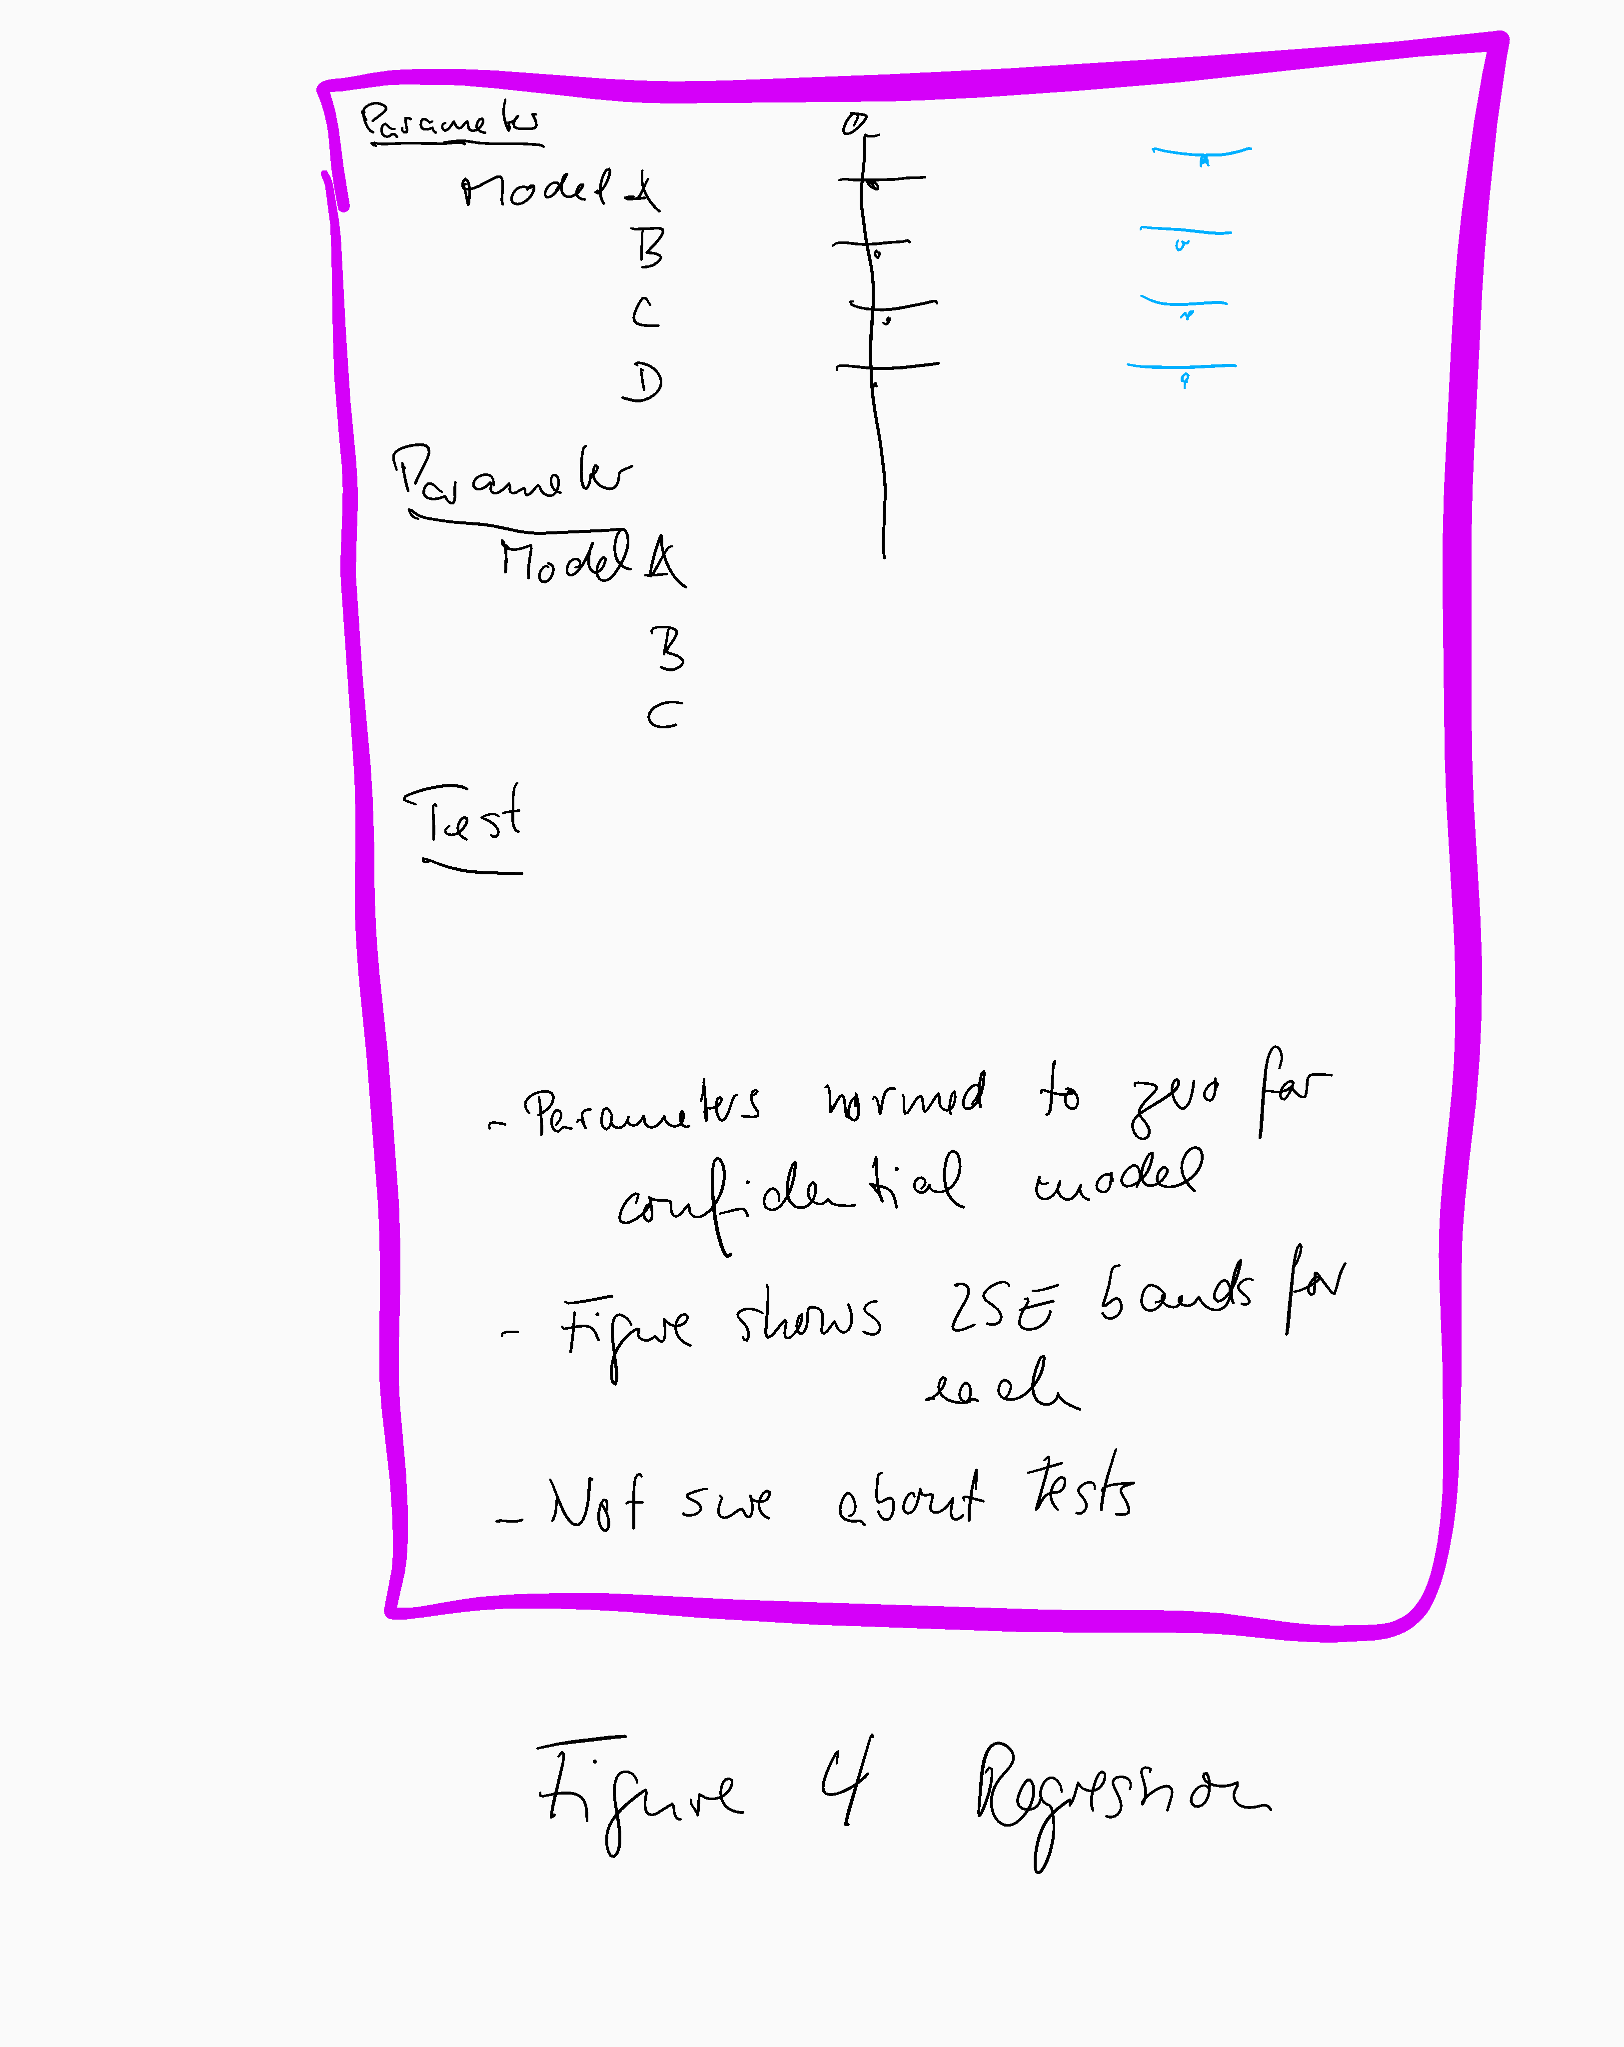
\includegraphics[width=.8\linewidth]{graphs/Figure4-placeholder.png} 
\caption{Alternate graph} 
\begin{minipage}{0.48\linewidth}
{\footnotesize To be computed in R. Detailed data are in the appendix. \par}
\end{minipage}
\end{figure}